\documentclass[12pt,a4paper]{article}

\usepackage[utf8]{inputenc}
\usepackage[T1]{fontenc}
\usepackage[provide=*,spanish]{babel}
\usepackage{amsmath,amssymb}
\usepackage{booktabs}
\usepackage{graphicx}
\usepackage{geometry}
\usepackage{xcolor}
\usepackage{url}
\usepackage{float}
\usepackage{array}

\geometry{margin=2.4cm}
\definecolor{outbreakgreen}{HTML}{567D35}
\definecolor{outbreakdark}{HTML}{18201B}
\definecolor{codebackground}{HTML}{F2F5F2}
\setlength{\parskip}{0.55em}
\setlength{\parindent}{0pt}

\title{\textbf{Outbreak: Stochastic Survival Lab}\\[0.4em]
\large Comparaci\'on de un proceso de Poisson y un proceso de renovaci\'on
generado mediante el m\'etodo polar}
\author{Estudiante(s): \rule{8cm}{0.4pt}\\
Curso de Modelaci\'on y Simulaci\'on\\
Docente: \rule{6cm}{0.4pt}}
\date{\today}

\begin{document}

\maketitle
\begin{figure}[H]
  \centering
  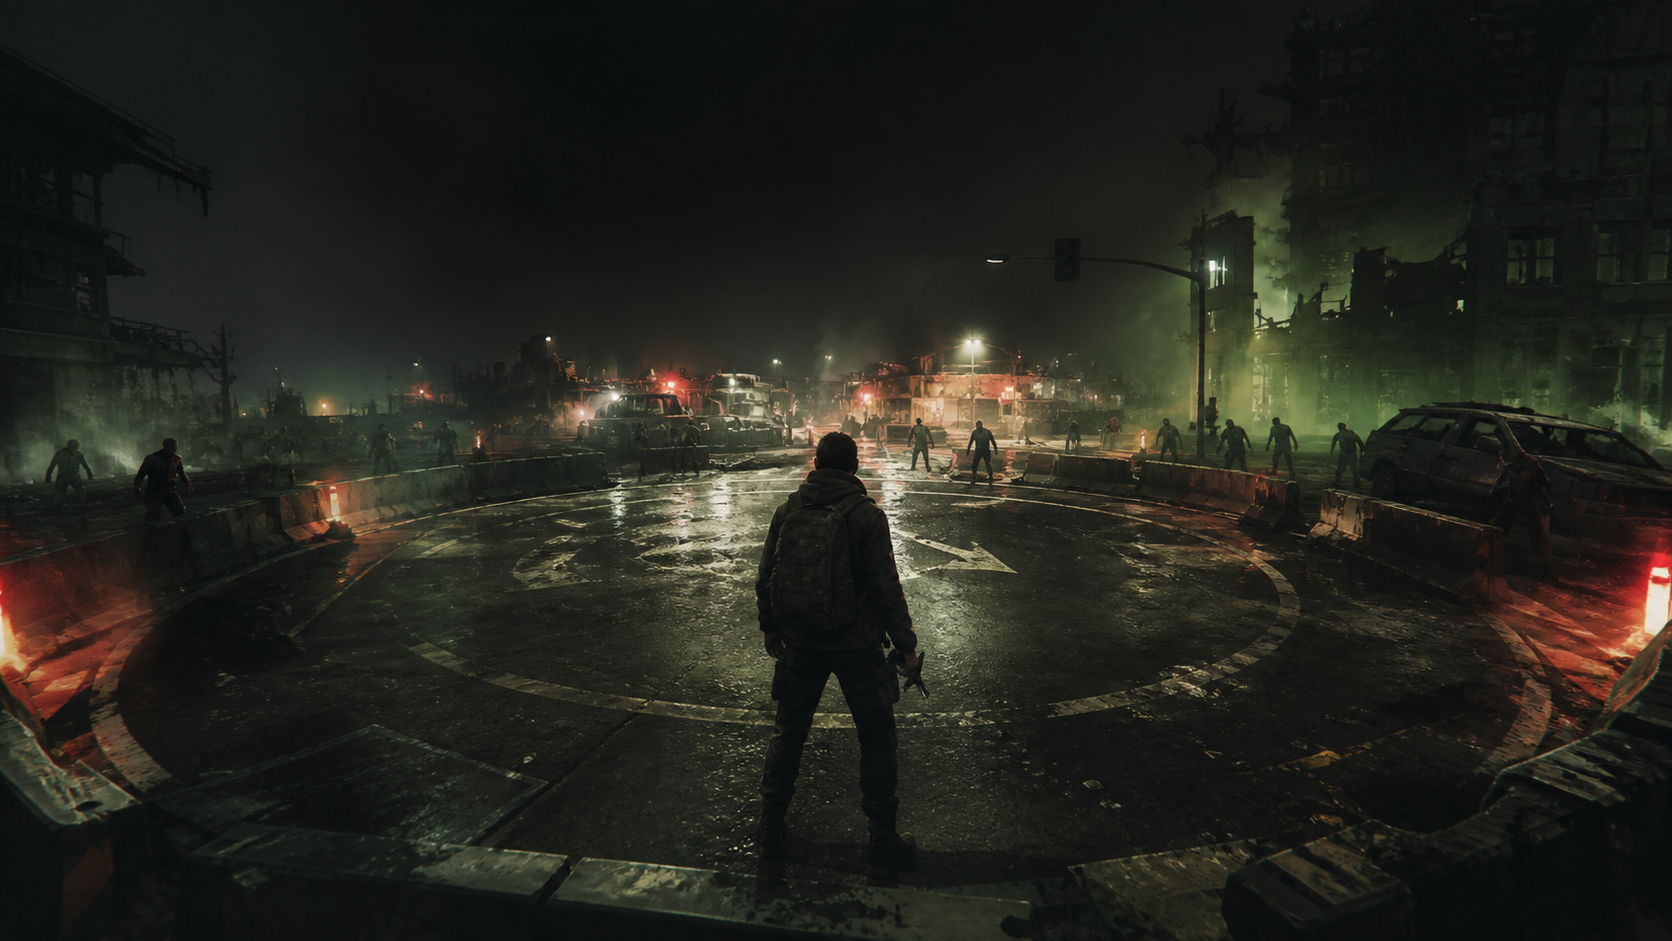
\includegraphics[width=0.96\textwidth]{assets/outbreak-command-center.png}
  \caption{Concepto visual de la zona de contenci\'on. Imagen generada para este proyecto.}
\end{figure}

\begin{abstract}
Este trabajo desarrolla una simulaci\'on estoc\'astica de supervivencia ante
infectados. Las llegadas se modelan principalmente mediante un proceso de
Poisson homog\'eneo, cuyos interarribos exponenciales se generan con transformada
inversa. Como contraste se implementa un proceso de renovaci\'on con interarribos
lognormales; las normales necesarias se obtienen con el m\'etodo polar de
Marsaglia. Ambos modelos se parametrizan con el mismo tiempo medio entre
llegadas. La din\'amica de combate se resuelve con paso temporal fijo y la
probabilidad de supervivencia se estima por Monte Carlo con intervalos de Wilson
al 95\,\%. La aplicaci\'on Streamlit integra controles, escena tridimensional
procedural, trazas temporales y experimentos reproducibles.
\end{abstract}

\tableofcontents
\newpage

\section{Introducci\'on}

En un videojuego de supervivencia, crear un enemigo cada cantidad fija de
segundos produce una secuencia predecible. Un modelo estoc\'astico representa
mejor la incertidumbre de una situaci\'on donde se conoce una frecuencia media,
pero no el instante exacto de la siguiente aparici\'on.

El proyecto estudia la relaci\'on entre esa incertidumbre y la supervivencia de
un protagonista. Adem\'as de una realizaci\'on individual, se ejecutan cientos de
partidas para cuantificar variabilidad y evitar conclusiones basadas en un caso
aislado.

\section{Planteamiento del problema}

\subsection{Pregunta de investigaci\'on}

\begin{quote}
\textit{\'C\'omo cambian la congesti\'on de enemigos y la probabilidad de
supervivencia cuando var\'ian la tasa y la distribuci\'on de los tiempos entre
llegadas?}
\end{quote}

\subsection{Objetivo general}

Modelar las apariciones aleatorias de infectados e integrar el proceso de
llegadas con reglas de movimiento y combate para estimar la probabilidad de que
el protagonista sobreviva un horizonte temporal finito.

\subsection{Objetivos espec\'ificos}

\begin{enumerate}
  \item Generar interarribos exponenciales mediante transformada inversa.
  \item Implementar el m\'etodo polar de Marsaglia y construir interarribos
        lognormales positivos.
  \item Comparar ambos modelos bajo una tasa media com\'un.
  \item Estimar probabilidades mediante Monte Carlo e informar incertidumbre.
  \item Visualizar el estado del sistema en una escena 3D interactiva.
  \item Garantizar reproducibilidad mediante semillas y pruebas automatizadas.
\end{enumerate}

\section{Fundamento matem\'atico}

\subsection{Proceso de Poisson homog\'eneo}

Sea $N(t)$ el n\'umero de llegadas hasta el tiempo $t$. Para una tasa constante
$\lambda>0$:

\begin{equation}
N(t)\sim\operatorname{Poisson}(\lambda t),
\end{equation}

\begin{equation}
P\{N(t)=k\}=e^{-\lambda t}\frac{(\lambda t)^k}{k!},
\qquad k=0,1,2,\ldots
\end{equation}

Una propiedad diagn\'ostica es la igualdad entre media y varianza:

\begin{equation}
\mathbb{E}[N(t)]=\operatorname{Var}[N(t)]=\lambda t.
\end{equation}

Los interarribos $\Delta_i$ son independientes y siguen una distribuci\'on
Exponencial$(\lambda)$:

\begin{equation}
f_{\Delta}(x)=\lambda e^{-\lambda x},\qquad x\geq 0.
\end{equation}

Si $U_i\sim U(0,1)$, la transformada inversa produce

\begin{equation}
\boxed{\Delta_i=-\frac{\ln(U_i)}{\lambda}}.
\end{equation}

Este modelo presenta falta de memoria y coeficiente de variaci\'on igual a uno;
por ello puede producir agrupaciones de llegadas y pausas largas.

\subsection{M\'etodo polar y alternativa lognormal}

El m\'etodo polar es un algoritmo de generaci\'on de normales, no un proceso de
llegadas. Se sortean $V_1,V_2\sim U(-1,1)$ y se calcula
$S=V_1^2+V_2^2$. Los pares con $S\notin(0,1)$ se rechazan. Para un par aceptado:

\begin{equation}
Z_1=V_1\sqrt{\frac{-2\ln S}{S}},\qquad
Z_2=V_2\sqrt{\frac{-2\ln S}{S}}.
\end{equation}

Ambos resultados siguen $N(0,1)$. Como un tiempo no puede ser negativo, se usa
la transformaci\'on lognormal

\begin{equation}
\Delta_i=\exp(\mu+\sigma Z_i).
\end{equation}

Sea $c$ el coeficiente de variaci\'on. Para conservar
$\mathbb{E}[\Delta]=1/\lambda$ se eligen

\begin{equation}
\sigma^2=\ln(1+c^2),\qquad
\mu=\ln(1/\lambda)-\frac{\sigma^2}{2}.
\end{equation}

Con $c<1$, las llegadas son m\'as regulares que en Poisson. El conteo resultante
es un proceso de renovaci\'on y no sigue, en general, una distribuci\'on Poisson.

\subsection{Acumulaci\'on de llegadas}

Para ambos modelos se construyen los instantes

\begin{equation}
t_0=0,\qquad t_i=t_{i-1}+\Delta_i.
\end{equation}

Se conservan aquellos $t_i$ dentro del horizonte de la misi\'on. Si el
protagonista cae antes del final, la telemetr\'ia de juego cuenta solamente las
llegadas ocurridas antes de la derrota; el calendario completo se mantiene por
separado para evitar la inconsistencia de la versi\'on inicial.

\section{Modelo de la simulaci\'on}

\subsection{Variables}

\begin{table}[H]
\centering
\caption{Clasificaci\'on de variables del sistema.}
\begin{tabular}{>{\bfseries}p{3.0cm}p{10.5cm}}
\toprule
Categor\'ia & Variables \\
\midrule
Entradas & $\lambda$, duraci\'on, modelo, CV, HP, DPS, alcance, velocidad,
paso temporal y semilla. \\
Estado & HP del jugador, enemigos activos, posiciones, HP individual y tiempo. \\
Aleatorias & Interarribos, \`angulo de aparici\'on, radio, velocidad, HP y DPS
de cada infectado. \\
Salidas & Supervivencia, tiempo resistido, llegadas, eliminados, remanentes y
pico de concurrencia. \\
\bottomrule
\end{tabular}
\end{table}

\subsection{Reglas operativas}

El protagonista permanece en el centro, ataca un objetivo a la vez y prioriza
al enemigo vivo m\'as cercano dentro de su alcance. Los infectados avanzan
radialmente. Al alcanzar el radio de contacto, sus tasas de da\~no se suman. La
misi\'on concluye al llegar al horizonte $T$ o cuando el HP llega a cero.

El tiempo se discretiza con $dt=0.05$ s por defecto. Reducir $dt$ disminuye el
error temporal a costa de mayor c\'omputo. El motor conserva una lista de
enemigos activos y evita recorrer, en cada paso, entidades que todav\'ia no han
aparecido.

\subsection{Par\'ametros base}

\begin{table}[H]
\centering
\caption{Escenario base reproducible.}
\begin{tabular}{lrr}
\toprule
Par\'ametro & Valor & Unidad \\
\midrule
Horizonte & 90 & s \\
Tasa & 39 & llegadas/min \\
CV Polar & 0.45 & adimensional \\
HP protagonista & 110 & HP \\
DPS protagonista & 42 & HP/s \\
Alcance & 10 & m \\
HP infectado & 42 & HP \\
Velocidad infectado & 1.55 & m/s \\
DPS infectado & 9 & HP/s \\
Paso temporal & 0.05 & s \\
Semilla & 22193 & --- \\
\bottomrule
\end{tabular}
\end{table}

\section{Dise\~no experimental}

Para una configuraci\'on fija se ejecutan $R$ partidas con semillas independientes.
Si $I_r$ vale uno cuando la partida $r$ termina con supervivencia:

\begin{equation}
\widehat p=\frac{1}{R}\sum_{r=1}^{R}I_r.
\end{equation}

La incertidumbre se expresa con un intervalo de Wilson al 95\,\%, preferido a la
aproximaci\'on normal simple cuando la proporci\'on est\'a cerca de cero o uno.

Para comparar modelos se utiliza una semilla maestra que produce el mismo vector
de semillas de corrida para Poisson y Polar-lognormal. Adem\'as, dentro de cada
partida se separa el flujo aleatorio de llegadas del flujo de atributos enemigos.
Este dise\~no pareado reduce diferencias accidentales.

\section{Resultados de referencia}

Se ejecutaron 400 partidas por modelo con el escenario base. La Tabla
\ref{tab:resultados} contiene resultados reproducibles con la versi\'on entregada.

\begin{table}[H]
\centering
\caption{Comparaci\'on Monte Carlo del escenario base, 400 partidas por modelo.}
\label{tab:resultados}
\begin{tabular}{lrrrr}
\toprule
Modelo & $\widehat p$ & IC 95\,\% & Tiempo medio (s) & Pico medio \\
\midrule
Poisson & 0.965 & [0.942, 0.979] & 88.526 & 9.483 \\
Polar-lognormal & 1.000 & [0.990, 1.000] & 90.000 & 6.483 \\
\bottomrule
\end{tabular}
\end{table}

Poisson produjo mayor concurrencia en este escenario, aunque ambos modelos
comparten una tasa media de 39 llegadas/min. El resultado se explica por la mayor
variabilidad exponencial: las rachas cortas elevan la presi\'on simult\'anea. El
modelo Polar-lognormal con $CV=0.45$ distribuye las llegadas de forma m\'as regular.

Estos resultados no significan que Polar sea siempre m\'as seguro ni que Poisson
sea ``mejor'' por producir determinada probabilidad. Poisson se considera el
modelo principal por su interpretabilidad, parsimonia y correspondencia con los
supuestos de llegadas independientes a tasa constante. Si los datos reales
mostraran regularidad o dependencia, otro proceso podr\'ia ser m\'as adecuado.

\section{Validaci\'on y verificaci\'on}

La entrega incluye nueve pruebas autom\'aticas:

\begin{itemize}
  \item reproducibilidad del generador y de la partida completa;
  \item cercan\'ia de media y varianza Poisson a $\lambda T$;
  \item media lognormal cercana a $1/\lambda$ y positividad;
  \item separaci\'on entre llegadas programadas y ocurridas tras una derrota;
  \item rechazo de geometr\'ias inv\'alidas;
  \item igualdad de semillas en la comparaci\'on pareada;
  \item estabilidad cualitativa al reducir $dt$;
  \item validez b\'asica del intervalo de Wilson.
\end{itemize}

Las pruebas se ejecutan con:

\begin{verbatim}
python -m unittest discover -s tests -v
\end{verbatim}

\section{Interfaz y tecnolog\'ia 3D}

Streamlit controla formularios, estado y cach\'e de experimentos. La simulaci\'on
solo se ejecuta cuando el usuario pulsa un bot\'on expl\'icito. Plotly representa
el terreno y mallas triangulares procedurales de personajes, edificios,
veh\'iculos y barricadas.

Pygame resulta apropiado para una aplicaci\'on de escritorio con superficies,
entrada y bucle de juego; el 3D requerir\'ia PyOpenGL y una ventana separada.
Panda3D es una alternativa futura para un ejecutable 3D independiente. Se eligi\'o
Plotly porque mantiene visualizaci\'on, controles y an\'alisis en la misma
aplicaci\'on web.

\section{Supuestos y limitaciones}

\begin{enumerate}
  \item La tasa es constante dentro de una partida.
  \item No existen colisiones entre infectados ni evitaci\'on de obst\'aculos.
  \item Las ruinas son parte visual del escenario y no modifican trayectorias.
  \item El protagonista es estacionario y enfoca un objetivo a la vez.
  \item El combate es una aproximaci\'on discreta dependiente de $dt$.
  \item El histograma de una sola misi\'on puede sufrir censura por el horizonte.
  \item Los resultados Monte Carlo dependen del escenario y del n\'umero de
        repeticiones; por eso se reportan intervalos de confianza.
\end{enumerate}

\section{Conclusiones}

El proyecto conecta una variable aleatoria continua con un mecanismo visible del
juego: cada interarribo determina cu\'anto falta para el siguiente infectado. El
proceso de Poisson ofrece una formulaci\'on directa, interpretable y verificable.
La comparaci\'on Polar-lognormal muestra que igualar solamente la tasa no iguala
la congesti\'on ni la supervivencia; la forma de la distribuci\'on tambi\'en importa.

La versi\'on final mejora la coherencia de telemetr\'ia, incorpora incertidumbre,
separa fuentes aleatorias, valida par\'ametros, optimiza el recorrido de entidades
y agrega pruebas. La escena 3D facilita la comunicaci\'on del modelo, mientras que
el informe y la interfaz dejan expl\'icitos los supuestos y l\'imites.

\section{Trabajo futuro}

Se propone estimar una tasa no homog\'enea $\lambda(t)$ para oleadas, permitir
movimiento del protagonista, incorporar colisiones y cobertura, calibrar
par\'ametros con datos observados y desarrollar una versi\'on independiente en
Panda3D con modelos animados y sonido.

\begin{thebibliography}{9}
\bibitem{ross}
S. M. Ross, \textit{Simulation}, Academic Press.

\bibitem{devroye}
L. Devroye, \textit{Non-Uniform Random Variate Generation}, Springer.

\bibitem{pygame}
Pygame Community, \textit{Pygame Documentation}.\\
\url{https://www.pygame.org/docs/}

\bibitem{panda3d}
Panda3D, \textit{Introduction to Panda3D}.\\
\url{https://docs.panda3d.org/1.10/python/introduction/index}

\bibitem{plotly}
Plotly, \textit{3D Mesh Plots in Python}.\\
\url{https://plotly.com/python/3d-mesh/}

\bibitem{streamlit}
Streamlit, \textit{Custom Components}.\\
\url{https://docs.streamlit.io/develop/concepts/custom-components}
\end{thebibliography}

\end{document}
